\PassOptionsToPackage{dvipsnames,svgnames,x11names}{xcolor}
\documentclass[tikz,border=8pt]{standalone}
\usetikzlibrary{arrows.meta,positioning,calc,shapes,shadows,decorations.pathmorphing,shapes.geometric,backgrounds,decorations.markings,decorations.pathreplacing,decorations.text,fit,shapes.misc,shapes.arrows,matrix,bending,3d,chains,intersections,shapes.symbols,svg.path,shapes.multipart,snakes,shapes.callouts,angles,quotes}
\providecolor{gold}{RGB}{212,175,55}
\providecolor{silver}{RGB}{192,192,192}
\providecolor{bronze}{RGB}{205,127,50}
\providecolor{darkblue}{RGB}{0,0,139}
\providecolor{lightblue}{RGB}{173,216,230}
\providecolor{darkgreen}{RGB}{0,100,0}
\providecolor{lightgreen}{RGB}{144,238,144}
\providecolor{darkred}{RGB}{139,0,0}
\providecolor{navy}{RGB}{0,0,128}
\providecolor{skyblue}{RGB}{135,206,235}
\providecolor{beige}{RGB}{245,245,220}
\providecolor{cream}{RGB}{255,253,208}
\usepackage{amsmath}
\usepackage{amssymb}
\usepackage{fontawesome5}
\usetikzlibrary{fadings,shadows.blur,patterns,patterns.meta}


\usepackage{amsmath}
\usepackage{amssymb}
\usepackage{fontawesome5}
\usepackage{tikz}
\usepackage{xcolor}

\providecolor{gold}{RGB}{212,175,55}
\providecolor{silver}{RGB}{192,192,192}
\providecolor{bronze}{RGB}{205,127,50}
\providecolor{darkblue}{RGB}{0,0,139}
\providecolor{lightblue}{RGB}{173,216,230}
\providecolor{darkgreen}{RGB}{0,100,0}
\providecolor{lightgreen}{RGB}{144,238,144}
\providecolor{darkred}{RGB}{139,0,0}
\providecolor{navy}{RGB}{0,0,128}
\providecolor{skyblue}{RGB}{135,206,235}
\providecolor{beige}{RGB}{245,245,220}
\providecolor{cream}{RGB}{255,253,208}

% --- CUSTOM COLORS ---
\definecolor{csscol}{RGB}{21, 101, 192}     % CSS Blue (#1565C0)
\definecolor{alertcol}{RGB}{211, 47, 47}    % Red for errors/blowouts (#D32F2F)
\definecolor{imgcol}{RGB}{76, 175, 80}      % Green for the image payload (#4CAF50)

\begin{document}
\begin{tikzpicture}[
    font=\sffamily,
    % --- STYLES ---
    bubble/.style={draw=gray!40, fill=white, rounded corners=6pt, inner sep=12pt, blur shadow={shadow opacity=20, shadow yshift=-2pt, shadow blur radius=4pt}, align=left},
    codebox/.style={fill=gray!10, draw=gray!30, font=\ttfamily\small, inner sep=10pt, rounded corners=4pt, align=left, blur shadow={shadow opacity=20, shadow yshift=-2pt, shadow blur radius=4pt}}
]

% Strict Pure White Background Bounding Box
\fill[white] (-1.5, -0.5) rectangle (25, 25);

% ==========================================
% 1. TITLE SECTION (ABSOLUTE POSITIONING)
% ==========================================
\node[font=\Huge\bfseries, text=black!80, align=center] at (11.5, 23.5) {The "Violent Override" in CSS Layout Tracks};
\node[font=\large, text=gray, align=center] at (11.5, 22.6) {Algorithmic conflict: Why an unconstrained $4000px$ image shatters a $300px$ Grid Column};

% ==========================================
% 2. LEFT SIDE: THE DEVELOPER'S INTENT
% ==========================================
\node[font=\Large\bfseries, text=csscol] at (4, 21.0) {1. The CSS Developer's Intent};

\node[codebox, anchor=north, text width=7.5cm] at (4, 20.0) {
{\color{gray}/* Define a strict 300px sidebar */}\\
.grid-container \{\\
\quad display: grid;\\
\quad \textbf{grid-template-columns: 300px 1fr;}\\
\}\\
{\color{gray}/* No constraints placed on the image */}\\
.sidebar img \{ \}\\
};

% Browser Label
\node[font=\footnotesize\bfseries, text=csscol] at (4, 11.0) {Intended Viewport / Grid Container (800px wide)};

% Browser Window Chrome (Left Base Frame)
\draw[gray!40, thick, rounded corners=4pt, fill=white] (0, 3) rectangle (8, 10.5);
\begin{scope}
    \clip[rounded corners=4pt] (0, 3) rectangle (8, 10.5);
    \fill[gray!15] (0, 9.75) rectangle (8, 10.5);
    \draw[gray!30] (0, 9.75) -- (8, 9.75);
    % macOS-style traffic light dots
    \fill[red!60] (0.4, 10.125) circle (2.2pt);
    \fill[yellow!60] (0.75, 10.125) circle (2.2pt);
    \fill[green!60] (1.1, 10.125) circle (2.2pt);
\end{scope}

% Track 1 (300px constraint)
\draw[fill=csscol!10, draw=csscol, thick] (0, 3) rectangle (3, 9.75);
\node[font=\bfseries\Large, text=csscol!90!black] at (1.5, 8.0) {300px};
\node[font=\footnotesize, text=gray!80!black] at (1.5, 7.3) {(.sidebar)};
\draw[dashed, csscol!80!black, thick, fill=csscol!5, rounded corners=2pt] (0.5, 3.5) rectangle (2.5, 5.5);
\node[font=\scriptsize\bfseries, text=csscol!80!black, align=center] at (1.5, 4.5) {Expected\\Image Box};

% Track 2 (1fr flexible remaining space)
\draw[fill=gray!10, draw=gray!40, thick] (3, 3) rectangle (8, 9.75);
\node[font=\bfseries\Large, text=gray!80!black] at (5.5, 7.3) {1fr (500px)};
\node[font=\footnotesize, text=gray] at (5.5, 6.6) {(.main-content)};

% Left Dimension Lines (Upper at y=2.0, Lower at y=1.0)
\draw[{Bar[width=4pt]}-{Bar[width=4pt]}, thick, csscol] (0, 2) -- (3, 2)
    node[midway, below, font=\scriptsize\bfseries, text=csscol] {300px};
\draw[{Bar[width=4pt]}-{Bar[width=4pt]}, thick, gray!70!black] (3, 2) -- (8, 2)
    node[midway, below, font=\scriptsize\bfseries, text=gray!70!black] {500px (1fr)};
\draw[{Bar[width=5pt]}-{Bar[width=5pt]}, thick, csscol!80!black] (0, 1) -- (8, 1)
    node[midway, below, font=\footnotesize\bfseries, text=csscol!80!black] {Total Intended Width: 800px};

% ==========================================
% 3. MIDDLE: THE INJECTION EVENT
% ==========================================
\node[font=\bfseries\small, align=center, text width=3.5cm, text=alertcol!90!black] at (10.0, 8.0)
    {Inject raw binary\\ \texttt{<img>}\\ ($4000 \times 3000$ px)};
\draw[-Stealth=3mm, line width=3pt, alertcol] (8.5, 6.5) -- (11.5, 6.5);

% ==========================================
% 4. RIGHT SIDE: THE DEVASTATING LAYOUT REALITY
% ==========================================
\node[font=\Large\bfseries, text=alertcol] at (17, 21.0) {2. The Devastating Layout Reality};

% The mechanism explanation bubble
\node[bubble, draw=alertcol, anchor=north, text width=8.5cm] at (17, 20.0) {
    \textbf{\color{alertcol}\faBomb \ The CSS Grid / Flex Minimums Rule}\vspace{2mm}\\
    By default, grid items do not shrink below their minimum content size (\texttt{min-width: auto}).\\
    For Replaced Elements (images), \texttt{auto} resolves directly to their \textbf{physical intrinsic size} ($4000px$).\\[2mm]
    \textbf{The layout engine calculates:}\\
    \textit{"Track 1 is commanded to be 300px, BUT its minimum required content size is 4000px. Because content prevents data loss by default, the track MUST violently expand to 4000px!"}
};

% Browser Label
\node[font=\footnotesize\bfseries, text=gray!80!black] at (16, 11.0) {Visible Viewport Window (800px) - User must now scroll};

% Browser Window Chrome (The Viewport Screen)
\draw[gray!50, thick, rounded corners=4pt, fill=white] (12, 3) rectangle (20, 10.5);
\begin{scope}
    \clip[rounded corners=4pt] (12, 3) rectangle (20, 10.5);
    \fill[gray!15] (12, 9.75) rectangle (20, 10.5);
    \draw[gray!30] (12, 9.75) -- (20, 9.75);
    % macOS-style traffic light dots
    \fill[red!60] (12.4, 10.125) circle (2.2pt);
    \fill[yellow!60] (12.75, 10.125) circle (2.2pt);
    \fill[green!60] (13.1, 10.125) circle (2.2pt);
\end{scope}

% Logical Layer 1: The Exploded Grid Container (Red Base) locked to [y=3.0 to y=9.75]
\draw[thick, alertcol, fill=alertcol!5]
    (12, 3) -- (12, 9.75) -- (23.0, 9.75)
    decorate [decoration={zigzag, segment length=6pt, amplitude=2pt}] { -- (23.0, 3) }
    -- cycle;

% Logical Layer 2: The Pushed 1fr Track (Gray) locked to [y=3.0 to y=9.75]
\draw[fill=gray!15, draw=gray!50, thick]
    (21.5, 3) -- (21.5, 9.75) -- (23.0, 9.75)
    decorate [decoration={zigzag, segment length=6pt, amplitude=2pt}] { -- (23.0, 3) }
    -- cycle;
\node[font=\scriptsize\bfseries, rotate=90, text=gray!80!black, align=center] at (22.25, 6.375) {1fr Track (Pushed off screen)};

% Logical Layer 3: The 4000px Image Box (Green) locked to [y=3.0 to y=9.75]
\draw[left color=imgcol!10, right color=imgcol!30, draw=imgcol, ultra thick]
    (12, 3) -- (12, 9.75) -- (21.5, 9.75)
    decorate [decoration={zigzag, segment length=6pt, amplitude=2pt}] { -- (21.5, 3) }
    -- cycle;

% Logical Layer 4: The Viewport Cutoff Line
\draw[thick, dashed, gray!70] (20, 3) -- (20, 10.5);

% Zero-Overlap Internal Image Text (Centered along x=16)
\node[font=\fontsize{42}{48}\selectfont, text=imgcol!35] at (16, 7.5) {\faImage};
\node[font=\LARGE\bfseries, text=imgcol!80!black, align=center] at (16, 6.0) {4000px\\Intrinsic Image};
\node[font=\bfseries\small, text=alertcol, fill=white, draw=alertcol, text width=7cm, align=center, inner sep=6pt, rounded corners=4pt, blur shadow={shadow opacity=20, shadow yshift=-2pt, shadow blur radius=4pt}] at (16, 4.5) {Track 1 minimum boundary forced to 4000px!};

% Floating LAYOUT OVERFLOW Warning Badge (Above viewport cutoff)
\draw[gray!50, thick, dashed] (20, 11.5) -- (20, 10.5);
\node[fill=white, draw=alertcol, line width=1.2pt, rounded corners=3pt, blur shadow={shadow opacity=20, shadow yshift=-2pt, shadow blur radius=4pt}, inner sep=5pt, align=center, anchor=south] at (20, 11.5) {
    {\color{alertcol}\large\faExclamationTriangle}\\[2pt]
    \textbf{\scriptsize\color{alertcol}LAYOUT OVERFLOW}\\[1pt]
    \tiny\color{gray!80!black}800px Viewport Exceeded
};

% Auxiliary Bottom Label (Pristine spacing at y=2.6)
\node[font=\footnotesize\bfseries, text=alertcol] at (17, 2.6) {Actual Rendered Grid Width (4000px + 1fr) $\rightarrow$ Horizontal Scroll of Death};

% Right Dimension Lines (Upper at y=2.0, Lower at y=1.0)
\draw[{Bar[width=5pt]}-{Bar[width=5pt]}, thick, gray!70!black] (12, 2) -- (20, 2)
    node[midway, below, font=\footnotesize\bfseries, text=gray!70!black] {Visible Viewport: 800px};
\draw[{Bar[width=5pt]}-, thick, alertcol] (12, 1) -- (23.0, 1)
    node[midway, below, font=\footnotesize\bfseries, text=alertcol] {Rendered Content: 4000px + 1fr (Horizontally Blown Out)};

\end{tikzpicture}
\end{document}
